\documentclass[10pt,a4paper]{article}
\usepackage[utf8]{inputenc}
\usepackage[T1]{fontenc}
\usepackage{amsmath}
\usepackage{amsfonts}
\usepackage{amssymb}
\usepackage{makeidx}
\usepackage{graphicx}
\usepackage{wrapfig}
\usepackage[left=1.00in, right=1.00in, top=1.00in, bottom=1.00in]{geometry}
\author{Tommaso Severini}
\title{Operone lac}
\begin{document}
	\maketitle
	
	In biologia, si definisce operone un insieme di geni regolati in modo strettamente correlato. Il più famoso tra questi è \textbf{l'operone lac}, noto per essere stato il primo esempio scoperto di controllo dell'espressione genica nei procarioti. La sua scoperta, da parte di  François Jacob e Jacques Monod, li ha portato a vincere il premio Nobel per la medicina nel 1965. Questo operone contiene i tre geni necessari al batterio Escherichia Coli per metabolizzare il lattosio, zucchero contenuto nel latte: \textbf{lacZ, lacY e lacA}. Questi geni codificano rispettivamente le proteine \textbf{$\beta-galattosidasi$}(sintesi allolattosio), che catalizza l'idrolisi dei residui terminali di $\beta-D-galattosio$ nelle molecole di lattosio scindendo lo zucchero i monosaccaridi, la \textbf{$lattosio permeasi$}, che permette alle molecole di lattosio di penetrare attraverso la membrana cellulare, e la \textbf{tiogalattoside transacetilasi}, che fornisce un gruppo acetile al $\beta-D-galattoside$ creato durante la digestione del lattosio anche se il suo ruolo non è stato ancora ben precisato.
	
	\section{La trascrizione dell'operone lac può essere repressa o attivata}	
	
	Quando E. coli si trova in un ambiente privo di lattosio, la sintesi dell'mRNA lac è repressa, in modo che la cellula non sprechi energia per sintetizzare proteine non utili al momento.
	\begin{wrapfigure}{r}{3in}
		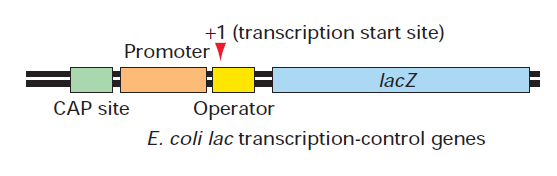
\includegraphics[width=2.5in]{operone.png}
	\end{wrapfigure}
	In un ambiente contenente sia glucosio che galattosio, la cellula preferisce prima metabolizzare il glucosio, molecola centrale nel metabolismo dei carboidrati. Il lattosio è metabolizzato a ritmi elevati solo quando il lattosio è presente e il glucosio è quasi del tutto assente. Questo equilibrio metabolico è ottenuto attraverso la repressione dell'operone lac fino a che il lattosio è presente , e la sintesi di bassi livelli di mRNA lac fino a che la concentrazione di glucosio nel citoplasma scende sotto livelli critici. La trascrizione dell'operone lac sotto diverse condizioni è controllato dal repressore e la proteina attivatrice da cataboliti, che si legano ad una specifica sequenza di DNA nella regione di controllo trascrizione dell'operone lac.
	
	\section{Assenza di lattosio}
	
	Quando il lattosio non è presente, il repressore si lega alla sequenza dell'operone detta \textbf{operatore}, che coincide con il punto di inizio della trascrizione, impedendo alla RNA polimerasi di iniziare la trascrizione.
	
	\begin{figure}[h]
		\centering
		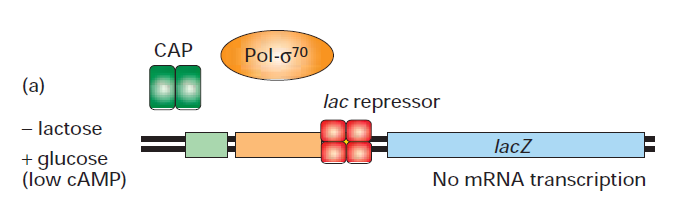
\includegraphics[width=0.7\textwidth]{operone no lac.png}	
	\end{figure}
	
	
	\section{Presenza di lattosio}
	
	Quando il lattosio è presente, un suo derivato ottenuto dall'azione della proteina $\beta-galattosidasi$, detto \textbf{allolattosio}, si lega al repressore, causandone un cambiamento di struttura che fa staccare il repressore dall'operatore. A causa di ciò, la polimerasi può iniziare la trascrizione dell'operone lac.
	
	La bassa concentrazione di glucosio fa in modo che le cellule di E. coli sintetizzino molta cAMP, adenosina monofosfato ciclico. Pian piano che la concentrazione di cAMP aumenta, essa si lega alla CAP, causandone una variazione conformazionale che gli permette di legarsi al sito dell'attivatore. Il complesso CAP-cAMP interagisce con la polimerasi, stimolando la produzione dell'mRNA.
	
	\begin{figure}[h]
		\centering
		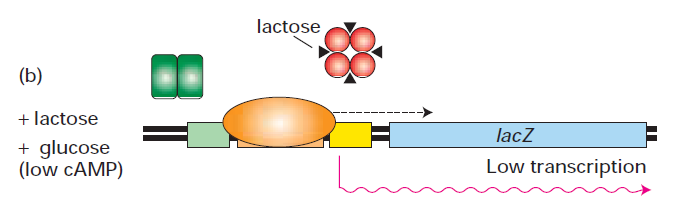
\includegraphics[width=0.7\textwidth]{operone si lac.png}
	\end{figure}
	
	
	\section{Presenza di lattosio e glucosio}
	
	Nonostante ciò, bisogna ricordare che, quando anche il glucosio è presente, il ritmo a cui la trascrizione avviene è molto minore, risultando nella sintesi di poche copie dell'mRNA lac e delle proteine codificate da quest'ultimo.
	
	\begin{figure}[h]
		\centering
		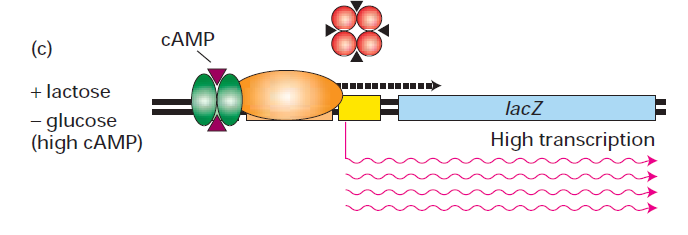
\includegraphics[width=0.7\textwidth]{operone no glu.png}
	\end{figure}
	
	
\end{document}